%%%%%%%%%%%%%%%%%%%%%%%%%%%%%%%%%%%%%%%%%%%%%%%%%%%%%%%%%%%%%%%%%%%%%%%%%%%%%%%%%%%%%%%%%%%%%%%%%%%
%%%%%%%%%%%%%%%%%%%%%%%%%%%%%%%%%%%%%%%%%%%%%%%%%%%%%%%%%%%%%%%%%%%%%%%%%%%%%%%%%%%%%%%%%%%%%%%%%%%
%%%%%%%%%%%%%%%%%%%%%%%%%%%%%%%%%%%%%%%%%%%%%%%%%%%%%%%%%%%%%%%%%%%%%%%%%%%%%%%%%%%%%%%%%%%%%%%%%%%
%%%%%%%%%%%%%%%%%%%%%%%%%%%%%%%%%%%%%%%%%%%%%%%%%%%%%%%%%%%%%%%%%%%%%%%%%%%%%%%%%%%%%%%%%%%%%%%%%%%
\documentclass{beamer}
\usepackage[utf8]{inputenc}
\usepackage[spanish]{babel}
\decimalpoint
\usepackage{amsmath}
\usepackage{amsfonts}
\usepackage{amssymb}
\usepackage{graphicx}

\usepackage{bibentry}

\usepackage{movie15}

\usepackage{verbatim}
%\usepackage{authblk}

\usepackage{listings}
\usepackage{color}

% para la bibliografia
\usepackage[style=verbose,backend=bibtex]{biblatex}

\bibstyle{abbrv}

% tachar texto
\usepackage{cancel}

% para las tablitas
\usepackage{booktabs}

% para tablas de colores
\usepackage{xcolor,colortbl}
\usepackage{multirow}

%%%%%%%%%%%%%%%%%%%%%%%%%%%%%%%%%%%%%%%%%%%%%%%%%%%%%%%%%%%%%%%%%%%%%%%%%%%%%%%%%%%%%%%%%%%%%%%%%%%
%%%%%%%%%%%%%%%%%%%%%%%%%%%%%%%%%%%%%%%%%%%%%%%%%%%%%%%%%%%%%%%%%%%%%%%%%%%%%%%%%%%%%%%%%%%%%%%%%%%

\addbibresource{referencias_estacionariedad.bib}
\addbibresource{referencias_fisiologia.bib}
\addbibresource{referencias_otros.bib}
\addbibresource{referencias_mixto.bib}

%%%%%%%%%%%%%%%%%%%%%%%%%%%%%%%%%%%%%%%%%%%%%%%%%%%%%%%%%%%%%%%%%%%%%%%%%%%%%%%%%%%%%%%%%%%%%%%%%%%
%%%%%%%%%%%%%%%%%%%%%%%%%%%%%%%%%%%%%%%%%%%%%%%%%%%%%%%%%%%%%%%%%%%%%%%%%%%%%%%%%%%%%%%%%%%%%%%%%%%

\newcommand{\bordes}[1]{\renewcommand{\arraystretch}{#1}}

\definecolor{gray}{rgb}{0.5,0.5,0.5}
\definecolor{gris}{gray}{0.925}
\definecolor{gris2}{gray}{0.8}

%%%%%%%%%%%%%%%%%%%%%%%%%%%%%%%%%%%%%%%%%%%%%%%%%%%%%%%%%%%%%%%%%%%%%%%%%%%%%%%%%%%%%%%%%%%%%%%%%%%
%%%%%%%%%%%%%%%%%%%%%%%%%%%%%%%%%%%%%%%%%%%%%%%%%%%%%%%%%%%%%%%%%%%%%%%%%%%%%%%%%%%%%%%%%%%%%%%%%%%

%\renewcommand{\bibfont}{\tiny}

%\renewcommand{\footnotesize}{\scriptsize}

\AtEveryCitekey{\iffootnote{\color{red}\scriptsize}{\color{blue}}}

%%%%%%%%%%%%%%%%%%%%%%%%%%%%%%%%%%%%%%%%%%%%%%%%%%%%%%%%%%%%%%%%%%%%%%%%%%%%%%%%%%%%%%%%%%%%%%%%%%%
%%%%%%%%%%%%%%%%%%%%%%%%%%%%%%%%%%%%%%%%%%%%%%%%%%%%%%%%%%%%%%%%%%%%%%%%%%%%%%%%%%%%%%%%%%%%%%%%%%%

%\usetheme{Luebeck}
\usetheme{CambridgeUS}
\usecolortheme{beaver}
{
%\usetheme{Luebeck}
%\setbeamercolor{palette secondary}{use=structure,fg=white,bg=red}
%\setbeamercolor{palette tertiary}{use=structure,fg=white,bg=green}
}

%
%
%
\definecolor{rojo}{rgb}{0.62353,0.10588,0.13725}
\definecolor{rojo2}{rgb}{0.32353,0.050588,0.06725}
\definecolor{naranja}{rgb}{0.91765,0.23137,0.16078}
\definecolor{rosa}{rgb}{0.95294,0.53333,0.32157}
\definecolor{cafe}{rgb}{0.48627,0.14118,0.10196}
\definecolor{cafe2}{rgb}{0.243135,0.07059,0.05098}
\definecolor{cafe3}{rgb}{0.1215675,0.035295,0.02549}

\definecolor{gris}{gray}{0.925}
\definecolor{gris2}{gray}{0.8}

\definecolor{UniBlue}{RGB}{83,121,170}
\setbeamercolor{title}{fg=white,bg=rojo}
\setbeamercolor{frametitle}{fg=white,bg=rojo}
\setbeamercolor{structure}{fg=rojo,bg=gris2}

\setbeamercolor{alerted text}{fg=rojo,bg=cafe2}
%\setbeamercolor{alerted text}{bg=cafe3,fg=white}

\setbeamercolor{palette primary}{bg=rojo2,fg=white}
%\setbeamercolor{palette secondary}{bg=cafe3,fg=white}
\setbeamercolor{palette tertiary}{bg=cafe2,fg=white}
\setbeamercolor{palette quaternary}{use=structure,bg=naranja,fg=white}
\setbeamercolor{itemize item}{bg=naranja,fg=naranja}
\setbeamercolor{section number projected }{bg=rosa,fg=white}

\setbeamertemplate{itemize item}{\color{naranja}$\bullet$}

%%%%%%%%%%%%%%%%%%%%%%%%%%%%%%%%%%%%%%%%%%%%%%%%%%%%%%%%%%%%%%%%%%%%%%%%%%%%%%%%%%%%%%%%%%%%%%%%%%%
%%%%%%%%%%%%%%%%%%%%%%%%%%%%%%%%%%%%%%%%%%%%%%%%%%%%%%%%%%%%%%%%%%%%%%%%%%%%%%%%%%%%%%%%%%%%%%%%%%%

%\DeclareUnicodeCharacter{00A0}{ }

\lstset{ %
%  language=R,                     % the language of the code
  basicstyle=\footnotesize,       % the size of the fonts that are used for the code
}

%%%%%%%%%%%%%%%%%%%%%%%%%%%%%%%%%%%%%%%%%%%%%%%%%%%%%%%%%%%%%%%%%%%%%%%%%%%%%%%%%%%%%%%%%%%%%%%%%%%
%%%%%%%%%%%%%%%%%%%%%%%%%%%%%%%%%%%%%%%%%%%%%%%%%%%%%%%%%%%%%%%%%%%%%%%%%%%%%%%%%%%%%%%%%%%%%%%%%%%

\newtheorem{defn}{Definici\'on}
\newtheorem{thrm}{Teorema}
\newtheorem{demostracion}{Demostraci\'on}
\newtheorem{prop}{Proposici\'on}

\newcommand{\R}{\mathbb{R}}
%\newcommand{\el2}{L^2}
\newcommand{\intR}{\int_{-\infty}^{\infty}}
\newcommand{\intZ}{\int_{-\infty}^{0}}
\newcommand{\intPI}{\int_{-\pi}^{\pi}}
\newcommand{\simint}[1]{\int_{- #1 }^{ #1 }}
\newcommand{\prima}{^{\prime}}

\newcommand{\ddd}{$\delta$}
\newcommand{\dirac}{$\delta$  de Dirac}

\newcommand{\aste}[1]{\widehat{ #1 }^{\star}}
\newcommand{\est}[1]{\widehat{ #1 }}

\newcommand{\COS}[1]{\mathrm{cos}\left( #1 \right)}
\newcommand{\SEN}[1]{\mathrm{sen}\left( #1 \right)}

\newcommand{\E}[1]{\mathrm{E}\left[ #1 \right]}
\newcommand{\Var}[1]{\mathrm{Var}\left( #1 \right)}
\newcommand{\Cov}[1]{\mathrm{Cov}\left( #1 \right)}
\newcommand{\abso}[1]{\left| #1 \right|}

%%%%%%%%%%%%%%%%%%%%%%%%%%%%%%%%%%%%%%%%%%%%%%%%%%%%%%%%%%%%%%%%%%%%%%%%%%%%%%%%%%%%%%%%%%%%%%%%%%%
%%%%%%%%%%%%%%%%%%%%%%%%%%%%%%%%%%%%%%%%%%%%%%%%%%%%%%%%%%%%%%%%%%%%%%%%%%%%%%%%%%%%%%%%%%%%%%%%%%%

\title[Estacionariedad en PSG de adultos mayores]
{Estacionariedad d\'ebil en registros de polisomnogr\'aficaos de adultos mayores,
como posible marcador de deterioro cognitivo}

\author[Enciso Alva]
{Julio Cesar Enciso Alva}

\institute[LIMA]
{Licenciatura en Matem\'aticas Aplicadas}

\date[Junio 2017]
{Seminario de investigaci\'on\\ Junio de 2017}

\titlegraphic{
\hspace*{8cm}~
\includegraphics[width=9em]{./material1/SIGLAS_UAEH_02.png}
}

%%%%%%%%%%%%%%%%%%%%%%%%%%%%%%%%%%%%%%%%%%%%%%%%%%%%%%%%%%%%%%%%%%%%%%%%%%%%%%%%%%%%%%%%%%%%%%%%%%%
%%%%%%%%%%%%%%%%%%%%%%%%%%%%%%%%%%%%%%%%%%%%%%%%%%%%%%%%%%%%%%%%%%%%%%%%%%%%%%%%%%%%%%%%%%%%%%%%%%%
%%%%%%%%%%%%%%%%%%%%%%%%%%%%%%%%%%%%%%%%%%%%%%%%%%%%%%%%%%%%%%%%%%%%%%%%%%%%%%%%%%%%%%%%%%%%%%%%%%%
%%%%%%%%%%%%%%%%%%%%%%%%%%%%%%%%%%%%%%%%%%%%%%%%%%%%%%%%%%%%%%%%%%%%%%%%%%%%%%%%%%%%%%%%%%%%%%%%%%%

%%%%%%%%%%%%%%%%%%%%%%%%%%%%%%%%%%%%%%%%%%%%%%%%%%%%%%%%%%%%%%%%%%%%%%%%%%%%%%%%%%%%%%%%%%%%%%%%%%%
%%%%%%%%%%%%%%%%%%%%%%%%%%%%%%%%%%%%%%%%%%%%%%%%%%%%%%%%%%%%%%%%%%%%%%%%%%%%%%%%%%%%%%%%%%%%%%%%%%%

\begin{document}

\frame{\titlepage}

%\begin{frame}
%\tableofcontents
%\end{frame}

%%%%%%%%%%%%%%%%%%%%%%%%%%%%%%%%%%%%%%%%%%%%%%%%%%%%%%%%%%%%%%%%%%%%%%%%%%%%%%%%%%%%%%%%%%%%%%%%%%%
%%%%%%%%%%%%%%%%%%%%%%%%%%%%%%%%%%%%%%%%%%%%%%%%%%%%%%%%%%%%%%%%%%%%%%%%%%%%%%%%%%%%%%%%%%%%%%%%%%%
%%%%%%%%%%%%%%%%%%%%%%%%%%%%%%%%%%%%%%%%%%%%%%%%%%%%%%%%%%%%%%%%%%%%%%%%%%%%%%%%%%%%%%%%%%%%%%%%%%%

\section{Introducci\'on}

%%%%%%%%%%%%%%%%%%%%%%%%%%%%%%%%%%%%%%%%%%%%%%%%%%%%%%%%%%%%%%%%%%%%%%%%%%%%%%%%%%%%%%%%%%%%%%%%%%%
%%%%%%%%%%%%%%%%%%%%%%%%%%%%%%%%%%%%%%%%%%%%%%%%%%%%%%%%%%%%%%%%%%%%%%%%%%%%%%%%%%%%%%%%%%%%%%%%%%%

\subsection{Antecedentes}

\begin{frame}\frametitle{Antecedentes}
\begin{itemize}
\item Encuesta Intercensal 2015 (INEGI): 12,500,000 adultos mayores, 10.4 \%  de la 
poblaci\'on %\footcite{Intercensal15}

\item Posible relaci\'on trastornos del sue\~no y DC en la vejez
%\footcite{Miyata13}

\item Epidemiolog\'ia del DC en Hidalgo: eficiencia del sue\~no%\footcite{VazquezTagle16}

\item DFA en registros de PSG:% \footcite{Valeria}: 
exponente de Hurst diferente en sujetos 
con y sin DC 

\item Se buscan marcadores cl\'inicos para el diagn\'ostico de DC
\end{itemize}
\end{frame}

%%%%%%%%%%%%%%%%%%%%%%%%%%%%%%%%%%%%%%%%%%%%%%%%%
%%%%%%%%%%%%%%%%%%%%%%%%%%%%%%%%%%%%%%%%%%%%%%%%%

%\begin{frame}\frametitle{El cuarteto de Anscombe}
%\begin{figure}
%\centering
%\includegraphics[width=0.9\linewidth]{anscombe.pdf} 
%\end{figure}
%\end{frame}

%%%%%%%%%%%%%%%%%%%%%%%%%%%%%%%%%%%%%%%%%%%%%%%%%%%%%%%%%%%%%%%%%%%%%%%%%%%%%%%%%%%%%%%%%%%%%%%%%%%
%%%%%%%%%%%%%%%%%%%%%%%%%%%%%%%%%%%%%%%%%%%%%%%%%%%%%%%%%%%%%%%%%%%%%%%%%%%%%%%%%%%%%%%%%%%%%%%%%%%

\subsection{Objetivos}

\begin{frame}\frametitle{Pregunta de investigaci\'on}
\textbf{
¿Es posible que la caracterizaci\'on de registros de actividad cerebral duarante el sue\~no, 
como series de tiempo d\'ebilmente 
estacionarias, pueda ser usada como un marcador en el diagn\'ostico cl\'inico para el dterioro 
cognitivo en adultos mayores?
}

\end{frame}

%%%%%%%%%%%%%%%%%%%%%%%%%%%%%%%%%%%%%%%%%%%%%%%%%
%%%%%%%%%%%%%%%%%%%%%%%%%%%%%%%%%%%%%%%%%%%%%%%%%

%\begin{frame}\frametitle{Objetivos}
%{\small
%\begin{description}
%%\textbf{General.} 
%\item[General:]
%Detectar, a partir de pruebas formales, las presencia de estacionariedad d\'ebil 
%en registros de PSG para adultos mayores% con y sin PDC
%
%%\textbf{Espec\'ificos} 
%\item[Espec\'ificos:]
%\begin{itemize}
%\item Estudiar la definici\'on de estacionariedad y sus implicaciones en un modelo
%
%\item Investigar c\'omo detectar si una serie de tiempo dada es estacionaria
%
%\item Determinar si los datos considerados son estacionarios
%\begin{itemize}
%\item Revisar si hay diferencias entre sujetos con y sin PDC
%\end{itemize}
%\end{itemize}
%\end{description}
%}
%\end{frame}

%%%%%%%%%%%%%%%%%%%%%%%%%%%%%%%%%%%%%%%%%%%%%%%%%%%%%%%%%%%%%%%%%%%%%%%%%%%%%%%%%%%%%%%%%%%%%%%%%%%
%%%%%%%%%%%%%%%%%%%%%%%%%%%%%%%%%%%%%%%%%%%%%%%%%%%%%%%%%%%%%%%%%%%%%%%%%%%%%%%%%%%%%%%%%%%%%%%%%%%
%%%%%%%%%%%%%%%%%%%%%%%%%%%%%%%%%%%%%%%%%%%%%%%%%%%%%%%%%%%%%%%%%%%%%%%%%%%%%%%%%%%%%%%%%%%%%%%%%%%

\section{Conceptos}

%%%%%%%%%%%%%%%%%%%%%%%%%%%%%%%%%%%%%%%%%%%%%%%%%%%%%%%%%%%%%%%%%%%%%%%%%%%%%%%%%%%%%%%%%%%%%%%%%%%
%%%%%%%%%%%%%%%%%%%%%%%%%%%%%%%%%%%%%%%%%%%%%%%%%%%%%%%%%%%%%%%%%%%%%%%%%%%%%%%%%%%%%%%%%%%%%%%%%%%

%\subsection{Fisiolog\'ia}
%
%\begin{frame}
%
%\frametitle{Conceptos}
%\begin{description}
%%\item[Adulto Mayor.] Individuo de 60 a\~nos o m\'as %\footcite{Hita14}.
%
%\item[Deterioro cognitivo leve\footnote{Usado como posible deterioro cognitivo (PDC)}.] 
%%\item[Deterioro cognitivo leve.] 
%Alteraci\'on adquirida y prolongada de funciones cognitivas; no s\'indrome focal, no demencia 
%%\footcite{Robles02}
%\item[Sue\~no.] Proceso vital c\'iclico complejo y activo%; caracter\'isticas:%\footcite{CarrilloMora}:
%\begin{description}
%\item[MOR ] Sue\~no parad\'ojico
%\begin{itemize}
%\item Movimientos oculares r\'apidos
%\item Aton\'ia muscular
%\item Actividad cerebral desincronizada
%
%\end{itemize}
%\item[NMOR] 
%\end{description}
%\end{description}
%\end{frame}

%%%%%%%%%%%%%%%%%%%%%%%%%%%%%%%%%%%%%%%%%%%%%%%%%%%%%%%%%%%%%%%%%%%%%%%%%%%%%%%%%%%%%%%%%%%%%%%%%%%
%%%%%%%%%%%%%%%%%%%%%%%%%%%%%%%%%%%%%%%%%%%%%%%%%%%%%%%%%%%%%%%%%%%%%%%%%%%%%%%%%%%%%%%%%%%%%%%%%%%

\subsection{Matem\'aticas}

\begin{frame}\frametitle{Conceptos}
%{\small
\begin{defn}[Estacionariedad d\'ebil]
%Se dice de un proceso estoc\'astico $\{ X(t) \}$ si (...)
%\begin{itemize}
%\item $\E{X(t)} = \E{X(t+\tau)}$
%\item $\E{X(t)X(s)} = \E{X(t+\tau)X(s+\tau)}$
%\end{itemize}
%\end{defn}
%
%\begin{thrm}
Un proceso estoc\'astico es d\'ebilmente estacionario si y s\'olo si %(...)
para cualesquiera tiempos admisibles $t$, $s$ se tiene que
\begin{itemize}
\item $\E{X(t)} = \mu_X$
\item $\Var{X(t)} = \sigma^{2}_X$
\item $\Cov{X(t),X(s)} = \rho_X (s-t)$
\end{itemize}
Con $\mu_X$, $\sigma^{2}_X$ constantes, $\rho_X(\tau)$ \'unicamente depende de $\tau$
%\end{thrm}
\end{defn}
%\emph{(...) = } para cualesquiera tiempos admisibles $t, s, t+\tau, s+\tau$
%}
\end{frame}

%%%%%%%%%%%%%%%%%%%%%%%%%%%%%%%%%%%%%%%%%%%%%%%%%
%%%%%%%%%%%%%%%%%%%%%%%%%%%%%%%%%%%%%%%%%%%%%%%%%

\begin{frame}\frametitle{Conceptos}
\begin{defn}[Continuidad estoc\'astica en media cuadr\'atica]
Un proceso a tiempo continuo $\{ X(t) \}$ es estoc\'asticamente continuo
en $t_0$ si y s\'olo si
\begin{equation*}
\lim_{t \rightarrow t_0} \E{\left( X\left(t\right) - X\left(t_0\right) \right)^{2}} = 0
\end{equation*}
\end{defn}

%\begin{figure}
%\includegraphics[width=.92\linewidth]{ehemplitos_ruido.png}
%\end{figure}
%\end{frame}
%
%%%%%%%%%%%%%%%%%%%%%%%%%%%%%%%%%%%%%%%%%%%%%%%%%%
%%%%%%%%%%%%%%%%%%%%%%%%%%%%%%%%%%%%%%%%%%%%%%%%%%
%
%\begin{frame}\frametitle{Conceptos}
\begin{defn}[Funci\'on de densidad espectral (SDF)]
Sea $\{X(t)\}$ un proceso estoc\'astico a tiempo continuo, d\'ebilmente estacionario
%\begin{equation*}
%h(\omega) = \lim_{T\rightarrow \infty} \E{ \frac{1}{2T} \frac{1}{2 \pi}
%\abso{ \int_{-T}^{T} X(t) e^{-i \omega t} dt}^{2} }
%\end{equation*}
\begin{equation*}
h(\omega) = \lim_{T\rightarrow \infty} \E{ \frac{ \left| G_T(\omega) \right|^{2}}{2 T} }
\end{equation*}
Donde $\displaystyle G_T (\omega) = \frac{1}{\sqrt{2 \pi}} \int_{-T}^{T} X(t) e^{-i \omega t} dt$
\end{defn}
\end{frame}

%%%%%%%%%%%%%%%%%%%%%%%%%%%%%%%%%%%%%%%%%%%%%%%%%
%%%%%%%%%%%%%%%%%%%%%%%%%%%%%%%%%%%%%%%%%%%%%%%%%

\begin{frame}%\frametitle{}
\begin{thrm}[Wiener-Khinchin]
Una condici\'on suficiente y necesaria para que
$\rho$ sea funci\'on de autocorrelaci\'on para alg\'un proceso a tiempo continuo d\'ebilmente 
estacionario y estoc\'asticamente continuo, $\{X(t)\}$,  es que exista una funci\'on $F$ tal que
\begin{itemize}
\item Es mon\'otonamente creciente
\item $F(-\infty) = 0$
\item $F(+\infty) = 1$
\item Para todo $\tau \in \R$ se cumple que
\begin{equation*}
\rho(\tau) = \intR e^{i \omega \tau} dF(\omega)
\end{equation*}
\end{itemize}
\end{thrm}
\end{frame}

%%%%%%%%%%%%%%%%%%%%%%%%%%%%%%%%%%%%%%%%%%%%%%%%%
%%%%%%%%%%%%%%%%%%%%%%%%%%%%%%%%%%%%%%%%%%%%%%%%%

\begin{frame}%\frametitle{}
\begin{thrm}[Wold]
Una condici\'on suficiente y necesaria para que $\rho$ sea funci\'on de autocorrelaci\'on para
alg\'un proceso estoc\'astico a tiempo discreto d\'ebilmente estacionario, $\{X(t)\}$, es que exista 
una funci\'on $F$ tal que
\begin{itemize}
\item Es mon\'otonamente creciente
\item $F(-\pi) = 0$
\item $F(+\pi) = 1$
\item Para todo $\tau \in \R$ se cumple que
\begin{equation*}
\rho(\tau) = \intPI e^{i \omega \tau} dF(\omega)
\end{equation*}
\end{itemize}
\end{thrm}
\end{frame}

%%%%%%%%%%%%%%%%%%%%%%%%%%%%%%%%%%%%%%%%%%%%%%%%%
%%%%%%%%%%%%%%%%%%%%%%%%%%%%%%%%%%%%%%%%%%%%%%%%%

\begin{frame}\frametitle{Representaci\'on de Wold-Cram\'er}
\begin{thrm}
Sea $\{X(t)\}$ un proceso a tiempo continuo, d\'ebilmente estacionario,
estoc\'asticamente continuo, de media 0 y 
varianza finita
Entonces, existe un proceso ortogonal $\{Z(\omega)\}$ tal que
\begin{equation*}
X(t) = \intR e^{i t \omega} dZ(\omega)
\end{equation*}
El proceso $\{Z(t)\}$ cumple para todo $\omega$
\begin{itemize}
\item $\E{dZ(\omega)} = 0$
\item $\E{\abso{dZ(\omega)}^{2}} = dH(\omega)$
\item $\Cov{dZ(\omega),dZ(\lambda)} = 0 \Leftrightarrow \omega \neq \lambda$
\end{itemize}
Con $H$ la SDF integrada de $\{X(t)\}$
\end{thrm}
\end{frame}

\begin{frame}\frametitle{Espectro evolutivo}
Se consideran procesos no-estacionarios, estoc\'asticamente continuos, de media cero y varianza finita,
y que admitan una representaci\'on de la forma
\begin{equation*}
X(t) = \intPI A(t,\omega) e^{i t \omega} dZ(\omega)
\end{equation*}
tal que 
\begin{itemize}
\item $\Cov{dZ(\omega),dZ(\lambda)} = 0 \Leftrightarrow \omega \neq \lambda$
\item $\E{\abso{dZ(\omega)}^{2}} = \mu(\omega)$
\end{itemize}

El \textbf{espectro evolutivo} fue definido por Priestley \footcite{Priestley65} como
\begin{equation*}
f(t,\omega) = \abso{A(t,\omega)}^{2}
\end{equation*}
% como el \textbf{espectro evolutivo}.
\end{frame}

%%%%%%%%%%%%%%%%%%%%%%%%%%%%%%%%%%%%%%%%%%%%%%%%%
%%%%%%%%%%%%%%%%%%%%%%%%%%%%%%%%%%%%%%%%%%%%%%%%%

\begin{frame}%\frametitle{Estimador de doble ventana}
%\begin{equation*}
%\{X(t)\} \text{  es d\'ebilmente estacionario}  \Rightarrow  f(t,\bullet) \text{  es constante}
%\end{equation*}
%Equivalentemente (contrapositiva):
%\begin{equation*}
%f(t,\bullet) \text{  \textbf{no} es constante} \Rightarrow  
%\{X(t)\} \text{  \textbf{no} es d\'ebilmente estacionario}  
%\end{equation*}
\begin{defn}[Estimador de doble ventana]
Se define a $\est{f}$, estimador para la $f$, como
\begin{equation*}
\widehat{f}(t,\omega) = \int_{t-T}^{t} w_{T'}(u) \lvert U(t-u,\omega) \lvert^{2} du
\end{equation*}
%con $U(t,\omega) = \int_{t-T}^{t} g(u) X({t-u}) e^{i \omega (t-u)} du$
%Donde $g$ y $w_\tau$, y sus ransformadas de Fourier $\Gamma$ y $W_\tau$, son tales que

\begin{itemize}
\item $U(t,\omega) = \int_{t-T}^{t} g(u) X({t-u}) e^{i \omega (t-u)} du$

\item $2\pi \int_{-\infty}^{\infty} \lvert g(u) \lvert^{2} du 
= 
\int_{-\infty}^{\infty} \lvert \Gamma(\omega) \lvert^{2} d\omega
= 1$
\item $w_{\tau}(t) \geq 0$ para cualesquiera $t$, $\tau$
\item $w_{\tau}(t) \rightarrow 0$ cuando $\lvert t \lvert \rightarrow \infty$, para todo $\tau$
\item $\int_{-\infty}^{\infty} w_{\tau}(t) dt = 1$ para todo $\tau$
\item $ \int_{-\infty}^{\infty} \left( w_{\tau}(t) \right)^{2} dt < \infty$ para todo $\tau$
\item $\exists C$ tal que  
$ \lim_{\tau\rightarrow\infty} \tau \int_{-\infty}^{t} \abso{ W_{\tau}(\lambda) }^{2} d\lambda = C$
\end{itemize}
\end{defn}
\end{frame}

%%%%%%%%%%%%%%%%%%%%%%%%%%%%%%%%%%%%%%%%%%%%%%%%%
%%%%%%%%%%%%%%%%%%%%%%%%%%%%%%%%%%%%%%%%%%%%%%%%%

\begin{frame}%\frametitle{}
\begin{prop}
El estimador de doble ventana $\widehat{f}$ tiene las siguientes propiedades
\begin{itemize}
\item $\displaystyle \E{\est{f}(t,\omega)} \approx f(t,\omega)$
\item $\displaystyle \Var{\est{f}(t,\omega)} \approx 
\frac{C}{\tau} f^{2}(t,\omega) \intR \abso{\Gamma (\theta)}^{4} d\theta$
\item $\displaystyle \Cov{\est{f}(t_1,\omega_1) , \est{f}(t_2,\omega_2)} \approx \intR \intR
w_\tau (u) w_\tau(v) \Cov{ \abso{U(t_1-u,\omega_1)}^{2} , \abso{U(t_2-u,\omega_2)}^{2} }
du dv$
\end{itemize}
\end{prop}

\begin{prop}
El estimador $ Y(t,\omega) = \log{\left( \est{f}(t,\omega)\right)}$
tiene las siguientes propiedades:
\begin{itemize}
\item $\displaystyle 
\E{ Y(t,\omega) } \approx \log \left( f(t,\omega) \right)$
\item $\displaystyle 
\Var{ Y(T,\omega) } 
\approx \frac{C}{\tau} \intR \abso{\Gamma (\theta)}^{4} d\theta $
\end{itemize}
\end{prop}
\end{frame}

%%%%%%%%%%%%%%%%%%%%%%%%%%%%%%%%%%%%%%%%%%%%%%%%%
%%%%%%%%%%%%%%%%%%%%%%%%%%%%%%%%%%%%%%%%%%%%%%%%%

\begin{frame}%\frametitle{}

M\'as a\'un, puede escribirse
\begin{equation*}
Y(t,\omega) = \log \left( f(t,\omega) \right) + \varepsilon(t,\omega)
\end{equation*}
donde las variables $\varepsilon(t,\omega)$ satisfacen que
\begin{itemize}
\item $\displaystyle \E{\varepsilon(t,\omega)} = 0$
\item $\displaystyle \Var{\varepsilon(t,\omega)}
\approx \frac{C}{\tau} \intR \abso{\Gamma (\theta)}^{4} d\theta$
\end{itemize}

En particular, se puede usar num\'ericamente el que
\begin{equation*}
\sum_{i = 1 }^{N} \left( Y(t,\omega_i) - \overline{Y}(\bullet,\omega_i) \right)^{2} 
\sim \sigma^{2} \chi^{2}(N)
\end{equation*}
con $\sigma^{2} = \Var{\varepsilon(t,\omega)}$, y
$\overline{Y}(\bullet,\omega) = \frac{1}{M} \sum_{j=1}^{M} Y(t_j,\omega)$.
\end{frame}

%%%%%%%%%%%%%%%%%%%%%%%%%%%%%%%%%%%%%%%%%%%%%%%%%
%%%%%%%%%%%%%%%%%%%%%%%%%%%%%%%%%%%%%%%%%%%%%%%%%

\begin{frame}[fragile]

\begin{figure}
\centering
\begin{lstlisting}
Priestley-Subba Rao stationarity Test for datos
-----------------------------------------------
Samples used              : 3072 
Samples available         : 3069 
Sampling interval         : 1 
SDF estimator             : Multitaper 
  Number of (sine) tapers : 5 
  Centered                : TRUE 
  Recentered              : FALSE 
Number of blocks          : 11 
Block size                : 279 
Number of blocks          : 11 
p-value for T             : 0.4130131 
p-value for I+R           : 0.1787949 
p-value for T+I+R         : 0.1801353 
\end{lstlisting}
\caption{La prueba de Priesltey-Subba Rao se encuentra implementada en R
como la sunci\'on \texttt{stationarity()}, del paquete \texttt{fractal}}
\end{figure}
\end{frame}

%%%%%%%%%%%%%%%%%%%%%%%%%%%%%%%%%%%%%%%%%%%%%%%%%
%%%%%%%%%%%%%%%%%%%%%%%%%%%%%%%%%%%%%%%%%%%%%%%%%

%\begin{frame}%\frametitle{}
%
%\end{frame}

%%%%%%%%%%%%%%%%%%%%%%%%%%%%%%%%%%%%%%%%%%%%%%%%%
%%%%%%%%%%%%%%%%%%%%%%%%%%%%%%%%%%%%%%%%%%%%%%%%%

%\begin{frame}%\frametitle{}
%\begin{prop}
%Sea $\{ X(t) \}$ un proceso d\'ebilmente estacionario, cuya funci\'on de autocovarianza es $R$, y
%sean $x_1, x_2 , \dots, x_N$ tales que $x_n$ es una observaci\'on de $X(n \Delta_{\tau})$) para
%alg\'un $\Delta_{\tau}$.
%El estimador para $R$ calculado como
%\begin{equation*}
%\aste{R}(\tau) = \frac{1}{N} 
%\sum_{t = 1}^{N-\abso{\tau}} x_t x_{t+\abso{\tau}}
%\end{equation*}
%tiene las siguientes propiedades:
%\begin{itemize}
%\item $\E{\aste{R}(\tau)} = \left(1 - \frac{\abso{\tau}}{N} \right) R(\omega)$
%\item $\Var{\aste{R}(\tau)} \approx \frac{1}{N} 
%\sum_{r=-\infty}^{\infty} \left( R^{2}(r) + R(r-\tau)R(r+\tau) \right)$
%\end{itemize}
%\end{prop}
%\end{frame}

%%%%%%%%%%%%%%%%%%%%%%%%%%%%%%%%%%%%%%%%%%%%%%%%%
%%%%%%%%%%%%%%%%%%%%%%%%%%%%%%%%%%%%%%%%%%%%%%%%%

%\begin{frame}%\frametitle{}
%\begin{defn}[Periodograma]
%Sean $x_1, x_2 , \dots, x_N$ observaciones de un proceso estoc\'astico de media cero y varianza
%finita. Se llama periodograma a la funci\'on $I_N: [-\pi,\pi] \rightarrow \R$ calculada como
%\begin{equation*}
%I_N(\omega) = \frac{2}{N} \abso{ \sum_{t=0}^{N} e^{i \omega t} x_t }^{2}
%\end{equation*}
%\end{defn}
%\begin{prop}
%Sean $x_1, x_2 , \dots, x_N$ observaciones de un proceso estoc\'astico de media cero y varianza
%finita. Se puede calcular el periodograma para estos datos como
%\begin{equation*}
%I_N(\omega) = 2 \sum_{r = -(N-1)}^{N-1} \aste{R}(r) \COS{r \omega}
%\end{equation*}
%\end{prop}
%\end{frame}

%%%%%%%%%%%%%%%%%%%%%%%%%%%%%%%%%%%%%%%%%%%%%%%%%
%%%%%%%%%%%%%%%%%%%%%%%%%%%%%%%%%%%%%%%%%%%%%%%%%

%\begin{frame}\frametitle{Periodograma: inconsistente}
%\begin{prop}
%Sea $\{X(t)\}$ un proceso d\'ebilmente estacionario com media cero, varianza finita y 
%espectro no puramente discreto; para cada $N$
%sean $x_1, x_2 , \dots, x_N$ observaciones del mismo y $I_N$ su periodograma. Entonces
%\begin{equation*}
%\lim_{N\rightarrow \infty} \Var{I_N(\omega)} = h^{2}(\omega)
%\end{equation*}
%\end{prop}
%
%\end{frame}

%%%%%%%%%%%%%%%%%%%%%%%%%%%%%%%%%%%%%%%%%%%%%%%%%
%%%%%%%%%%%%%%%%%%%%%%%%%%%%%%%%%%%%%%%%%%%%%%%%%

%\begin{frame}%\frametitle{}
%
%\end{frame}

%%%%%%%%%%%%%%%%%%%%%%%%%%%%%%%%%%%%%%%%%%%%%%%%%%%%%%%%%%%%%%%%%%%%%%%%%%%%%%%%%%%%%%%%%%%%%%%%%%%
%%%%%%%%%%%%%%%%%%%%%%%%%%%%%%%%%%%%%%%%%%%%%%%%%%%%%%%%%%%%%%%%%%%%%%%%%%%%%%%%%%%%%%%%%%%%%%%%%%%

\section{Metodolog\'ia}

\subsection{Conceptos, fisiolog\'ia}

\begin{frame}

\frametitle{Conceptos}
\begin{description}
%\item[Adulto Mayor.] Individuo de 60 a\~nos o m\'as %\footcite{Hita14}.

\item[Deterioro cognitivo leve\footnote{Usado como posible deterioro cognitivo (PDC)}] 
%\item[Deterioro cognitivo leve.] 
Alteraci\'on adquirida y prolongada de funciones cognitivas; no s\'indrome focal, no demencia 
%\footcite{Robles02}
\item[Sue\~no] Proceso vital c\'iclico complejo y activo%; caracter\'isticas:%\footcite{CarrilloMora}:
%\begin{description}
\item[S. MOR] Fase m\'as profunda, alta actividad cerebral, se producen enso\~naciones, \textit{sue\~no parad\'ojico}
\begin{itemize}
\item Movimientos oculares r\'apidos
\item Aton\'ia muscular
\item Actividad cerebral desincronizada

\end{itemize}
%\end{description}
\end{description}
\end{frame}

\subsection{Sujetos}

\begin{frame}\frametitle{Sujetos}
Criterios de inclusi\'on:
\begin{itemize}
\item Firma del consentimiento informado
\item Edad entre 60 y 85 a\~nos
\item Diestros (mano derecha dominante)
\item Sin ansiedad, depresi\'on o s\'indromes focales
\item No usar medicamentos o sustancias para dormir
\item Voluntario para el registro de PSG
\end{itemize}

\textbf{9 participantes: 4 control, 5 PDC}
\end{frame}

%%%%%%%%%%%%%%%%%%%%%%%%%%%%%%%%%%%%%%%%%%%%%%%%%
%%%%%%%%%%%%%%%%%%%%%%%%%%%%%%%%%%%%%%%%%%%%%%%%%

\begin{frame}\frametitle{Sujetos}
\begin{table}
\centering
\bordes{1.1}
\begin{tiny}
\begin{tabular}{llcrrrrrrr}
\toprule
 \phantom{mm}&
 & \textbf{Sexo} & \textbf{Edad} & \textbf{Esc.} & \textbf{Neuropsi} & \textbf{MMSE} & \textbf{SATS} & \textbf{KATZ} & \textbf{Gds} \\
\midrule
\multicolumn{6}{l}{\textbf{Gpo. Control}}\\
&VCR    & F    & 59   & 12   & 107      & 29   & 21   & 0    & 3 \\
&MJH    & F    & 72   & 9    & 113      & 30   & 18   & 0    & 0 \\
&JAE    & F    & 78   & 5    & 102      & 28   & 19   & 0    & 5 \\
&GHA    & M    & 65   & 9    & 107.5    & 30   & 23   & 0    & 7 \\
&MFGR   & F    & 67   & 11   & 110      & 30   & 18   & 0    &   \\
\rowcolor{gris}
&\multicolumn{1}{c}{$\widehat{\mu}$} & 
              & 68.20& 9.20 & 107.90   & 29.40& 19.80& 0.00 & 3.00\\
\rowcolor{gris}
&\multicolumn{1}{c}{$\widehat{\sigma}$} & 
              & 7.19 & 2.68 & 4.07     & 0.89 & 2.17 & 0.00 & 3.08\\
\midrule
%\hline
\multicolumn{6}{l}{\textbf{Gpo. PDC}}\\
&CLO    & F    & 68   & 5    & 81       & 28   & 22   & 1    & 6 \\
&RLO    & F    & 63   & 9    & 90       & 29   & 20   & 0    & 3 \\
&RRU    & M    & 69   & 9    & 85       & 27   & 10   & 0    & 3 \\
&JGZ    & M    & 65   & 11   & 87       & 25   & 20   & 0    & 1 \\
\rowcolor{gris}
&\multicolumn{1}{c}{$\widehat{\mu}$} & 
              & 66.25& 8.50 & 85.75   & 27.25& 18.00& 0.25 & 3.25\\
\rowcolor{gris}
&\multicolumn{1}{c}{$\widehat{\sigma}$} & 
              & 2.75 & 2.52 & 3.77    & 1.71 & 5.42 & 0.50 & 2.06\\
\midrule
%\hline
\multicolumn{6}{l}{\textbf{Sujetos excluidos}}\\
&FGH    & M    & 71   & 9    & 83.5     & 21   & 23   & 0    & 4  \\
&MGG    & F    & 61   & 9    & 114      & 28   & 29   & 1    & 14 \\
&EMT    & M    & 50   & 22   & 106      & 30   & 15   & 0    & 4  \\
\bottomrule
\end{tabular} 
\end{tiny}
%\caption{Resultados de las pruebas neuropsicol\'ogicas aplicadas a los sujetos considerados en este 
%trabajo, adem\'as de algunos datos generales. 
%}
\end{table}
\end{frame}

%%%%%%%%%%%%%%%%%%%%%%%%%%%%%%%%%%%%%%%%%%%%%%%%%
%%%%%%%%%%%%%%%%%%%%%%%%%%%%%%%%%%%%%%%%%%%%%%%%%

\begin{frame}\frametitle{Registro de PSG}
\begin{figure}
\centering
%\begin{tabular}{cc}
%\includegraphics[height=15em]{foto_registro.jpg} 
%& 
%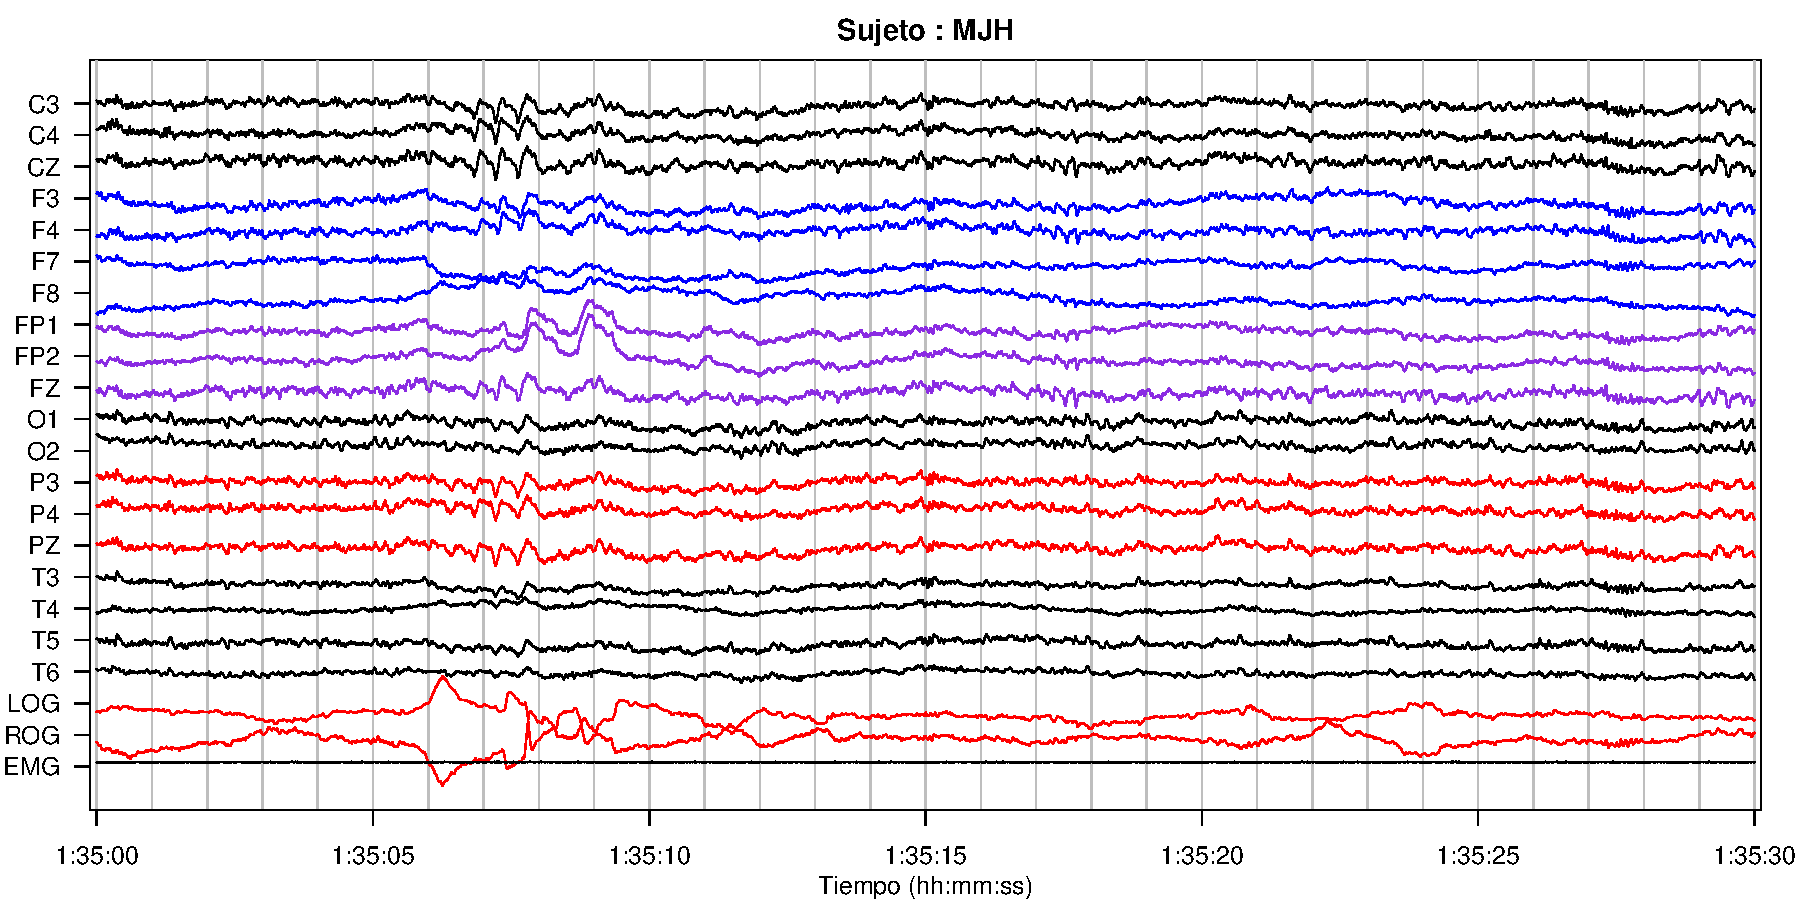
\includegraphics[height=10em]{./p_170427/MJH_190_PDG_lucirse_PSG.pdf}
%\\
%\end{tabular}
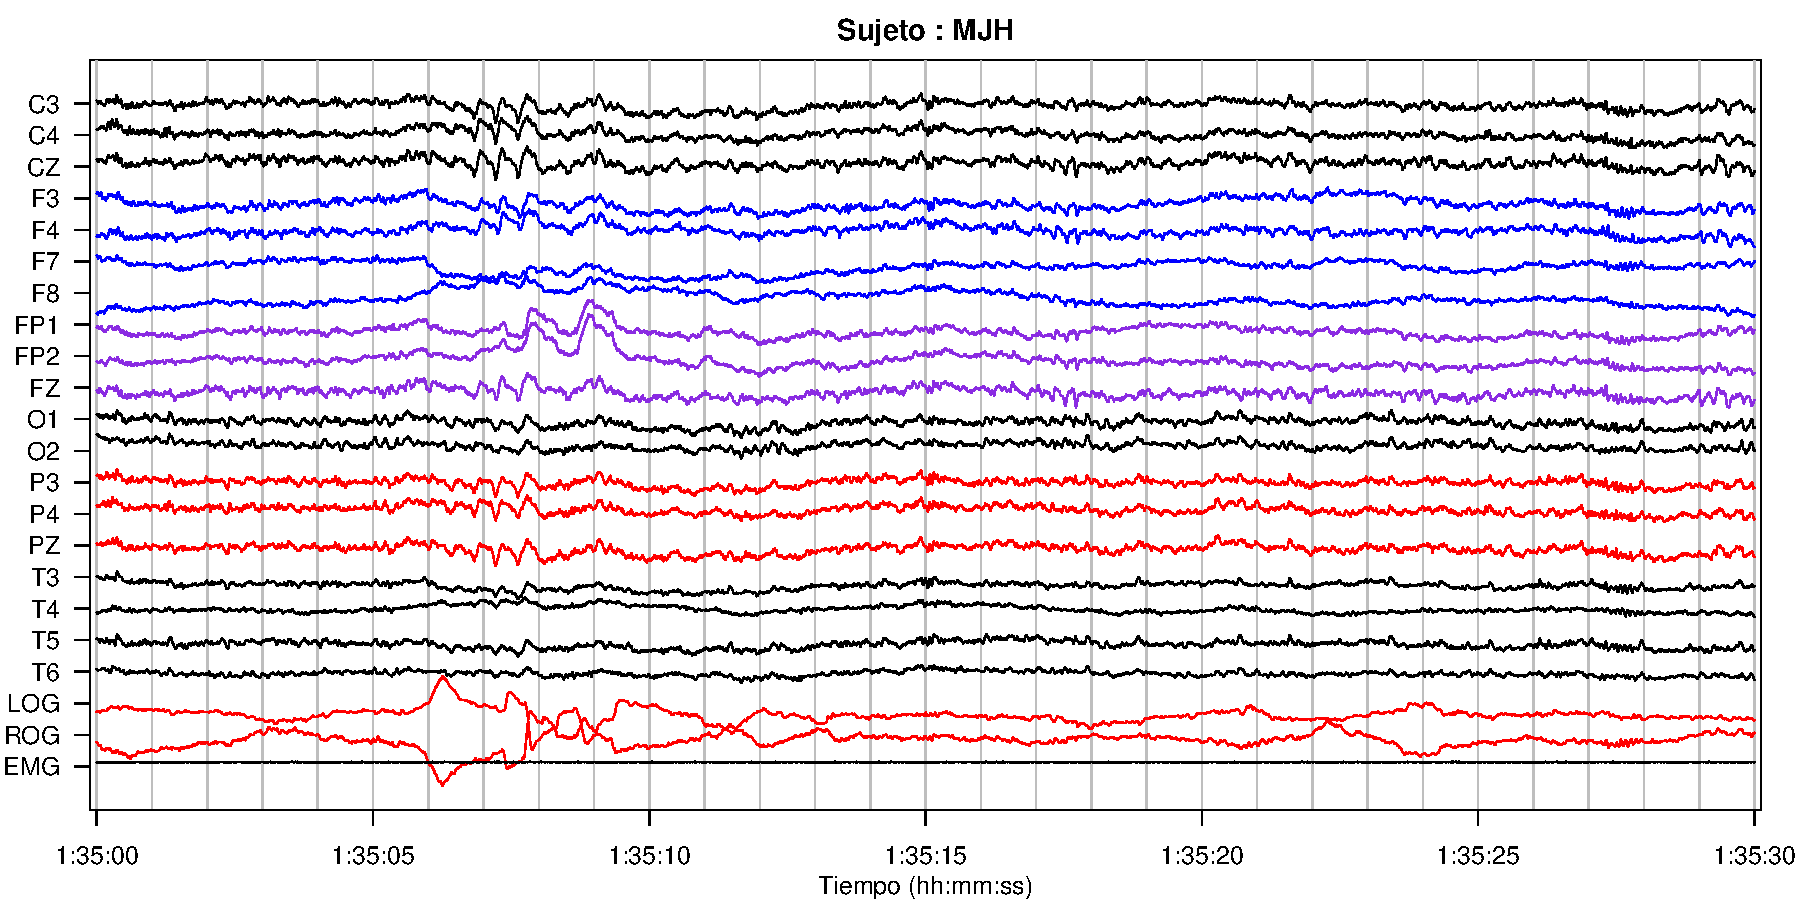
\includegraphics[width=0.9\linewidth]{./p_170427/MJH_190_PDG_lucirse_PSG.pdf}
\caption{PSG: 19 electrodos EEG, 4 electrodos EOG (horizontal y vertical), 2 electrodos EMG en 
m\'usculos submentonianos}
\end{figure}
\end{frame}

%%%%%%%%%%%%%%%%%%%%%%%%%%%%%%%%%%%%%%%%%%%%%%%%%
%%%%%%%%%%%%%%%%%%%%%%%%%%%%%%%%%%%%%%%%%%%%%%%%%

\begin{frame}\frametitle{PSG: EEG}
%\begin{description}
%\item[Electroencefalograma.] Registro de las fluctuaciones en potenciales el\'ectricos en el 
%cerebro
%\end{description}
\begin{figure}
\centering
\includegraphics[width=0.9\linewidth]{cabeza_hecha.pdf} 
\caption{Sistema de referencia 10--20}
\end{figure}
\end{frame}

%%%%%%%%%%%%%%%%%%%%%%%%%%%%%%%%%%%%%%%%%%%%%%%%%
%%%%%%%%%%%%%%%%%%%%%%%%%%%%%%%%%%%%%%%%%%%%%%%%%

\begin{frame}\frametitle{Registro de PSG}
\begin{table}
\centering
\bordes{1.1}
\begin{tiny}
\begin{tabular}{llcrrcrrr}
\toprule
    \phantom{mm}&
    &\multirow{2}{*}{\begin{tabular}{c}\bordes{1}Frecuencia\\ muestreo\end{tabular}}
    \bordes{1.2}
    & \multicolumn{2}{c}{Total} & \phantom{l}   & \multicolumn{3}{c}{MOR}\\
    \cmidrule{4-5}  \cmidrule{7-9}
    &&          &Puntos  &  Tiempo   &&Puntos  &  Tiempo   &  \% MOR \\
\midrule
\multicolumn{6}{l}{\textbf{Gpo. Control}}\\
&VCR &200       & 5166000&   7:10:30 &&438000  &   0:36:30 & 8\% \\
&MJH &512       &15851520&   8:36:00 &&1950720 &   1:03:30 &12\% \\
&JAE &512       &13931520&   7:33:30 &&2626560 &   1:25:30 &19\% \\
&GHA &200       &6558000 &   9:06:00 &&330000  &   0:27:30 & 5\% \\
&MFGR&200       &4932000 &   6:51:00 &&570000  &   0:47:30 &12\% \\

\midrule

\rowcolor{gris}
\multicolumn{9}{l}{\textbf{Gpo. PDC}}\\
\rowcolor{gris}
&CLO &512       &14499840&   7:52:00 &&2027520 &   1:06:00 &14\% \\
\rowcolor{gris}
&RLO &512       &12994560&   7:03:00 &&1520640 &   0:49:30 &12\% \\
\rowcolor{gris}
&RRU &200       &2484000 &   3:27:00 &&228000  &   0:19:00 & 9\% \\
\rowcolor{gris}
&JGZ &512       &18539520&  10:03:30 &&506880  &   0:16:30 & 3\% \\

\midrule

\multicolumn{6}{l}{\textbf{Sujetos excluidos}}\\
&FGH &512       &6220800 &   3:22:30 &&337920  &   0:11:00 & 5\% \\
&MGG &512       &15820800&   8:35:00 &&2549760 &   1:23:00 &16\% \\
&EMT &512       &21857280&  11:51:30 &&721920  &   0:23:30 & 3\% \\
\bottomrule
\end{tabular}
\end{tiny}
\end{table}
\end{frame}

%%%%%%%%%%%%%%%%%%%%%%%%%%%%%%%%%%%%%%%%%%%%%%%%%
%%%%%%%%%%%%%%%%%%%%%%%%%%%%%%%%%%%%%%%%%%%%%%%%%

%\begin{frame}%\frametitle{}
%
%\end{frame}

%%%%%%%%%%%%%%%%%%%%%%%%%%%%%%%%%%%%%%%%%%%%%%%%%%%%%%%%%%%%%%%%%%%%%%%%%%%%%%%%%%%%%%%%%%%%%%%%%%%
%%%%%%%%%%%%%%%%%%%%%%%%%%%%%%%%%%%%%%%%%%%%%%%%%%%%%%%%%%%%%%%%%%%%%%%%%%%%%%%%%%%%%%%%%%%%%%%%%%%

\section{Resultados}

\subsection{Resultados principales}

\begin{frame}\frametitle{Resultados principales}
\begin{itemize}
\item Cada \'epoca fue clasificada 'posiblemente estacionaria' (PE) no se rechaza la 
hip\'otesis de estacionariedad ($\alpha < 0.05$) en PSR

\item Debido a la variabilidad entre sujetos, se consider\'o la proporci\'on de \'epocas PE
en cada etapa
\begin{equation*}
\text{\% \'epocas PE} = \frac{\text{\# \'epocas PE en MOR}}{\text{\# \'epocas en MOR}}
\end{equation*}

\item Las proporciones se compararon:
\begin{itemize}
\item MOR vs NMOR (individual y grupal)
\item Grupo Control vs Grupo PDC (en cada etapa de sue\~no)
\end{itemize}
\end{itemize}
\end{frame}

%%%%%%%%%%%%%%%%%%%%%%%%%%%%%%%%%%%%%%%%%%%%%%%%%
%%%%%%%%%%%%%%%%%%%%%%%%%%%%%%%%%%%%%%%%%%%%%%%%%

\begin{frame}\frametitle{MOR vs NMOR, individual}
\begin{figure}
\centering
\begin{tabular}{c}
\begin{tabular}{ccccc}
\includegraphics[width=0.15\textwidth]{./cabecitas/cabecita_VCR.pdf} &
\includegraphics[width=0.15\textwidth]{./cabecitas/cabecita_MJH.pdf} &
\includegraphics[width=0.15\textwidth]{./cabecitas/cabecita_JAE.pdf} &
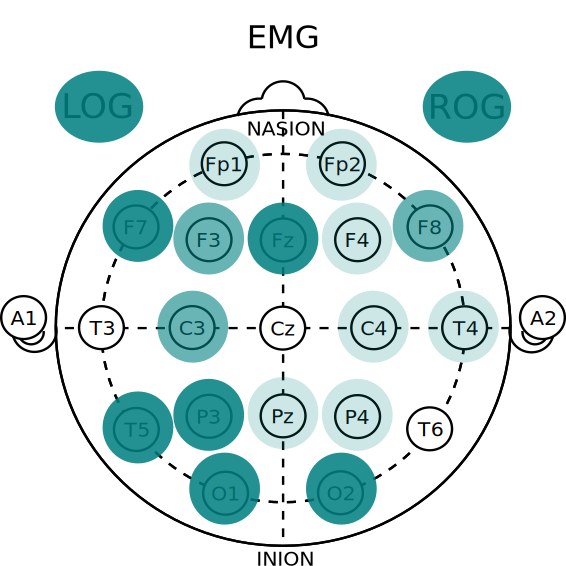
\includegraphics[width=0.15\textwidth]{./cabecitas/cabecita_GHA.pdf} &
\includegraphics[width=0.15\textwidth]{./cabecitas/cabecita_MFGR.pdf} \\
VCR & MJH & JAE & GHA & MFGR
\end{tabular}
\\
\begin{tabular}{cccc}
\includegraphics[width=0.15\textwidth]{./cabecitas/cabecita_CLO.pdf} &
\includegraphics[width=0.15\textwidth]{./cabecitas/cabecita_RLO.pdf} &
\includegraphics[width=0.15\textwidth]{./cabecitas/cabecita_RRU.pdf} &
\includegraphics[width=0.15\textwidth]{./cabecitas/cabecita_JGZ.pdf} \\
CLO & RLO & RRU & JGZ
\end{tabular}
\end{tabular}
\caption{En azul las zonas donde se encontraron diferencias significativas}
%\label{cabecitas_munchas}
\end{figure}
\end{frame}

%%%%%%%%%%%%%%%%%%%%%%%%%%%%%%%%%%%%%%%%%%%%%%%%%
%%%%%%%%%%%%%%%%%%%%%%%%%%%%%%%%%%%%%%%%%%%%%%%%%

\begin{frame}\frametitle{Gpo. Control vs Gpo. PDC}
\begin{figure}
\centering
\begin{tabular}{rl}
{\Large \textbf{MOR}}
&
\includegraphics[width=0.6\linewidth]
{./new170424/Comparacion_gpos_MOR.pdf} 
\\
{\Large \textbf{NMOR}}
&
\includegraphics[width=0.6\linewidth]
{./new170424/Comparacion_gpos_NMOR.pdf} 
\end{tabular}
\caption{ Promedio $\pm$ 1 desviaci\'on est\'andar. Control: azul, PDC: rojo.}
\end{figure}
\end{frame}

%%%%%%%%%%%%%%%%%%%%%%%%%%%%%%%%%%%%%%%%%%%%%%%%%
%%%%%%%%%%%%%%%%%%%%%%%%%%%%%%%%%%%%%%%%%%%%%%%%%

\begin{frame}\frametitle{MOR vs NMOR, grupal}
\begin{figure}
\centering
\begin{tabular}{rl}
{\Large \textbf{Gpo. Control}}
&
\includegraphics[width=0.6\linewidth]
{./new170424/comp_etapas_gpos_NORMALMOR_vs_NMOR.pdf} 
\\
{\Large \textbf{Gpo. PDC}}
&
\includegraphics[width=0.6\linewidth]
{./new170424/comp_etapas_gpos_PDCMOR_vs_NMOR.pdf} 
\end{tabular}
\caption{ Promedio $\pm$ 1 desviaci\'on est\'andar. MOR: verde, NMOR: negro.}
\end{figure}
\end{frame}

%%%%%%%%%%%%%%%%%%%%%%%%%%%%%%%%%%%%%%%%%%%%%%%%%
%%%%%%%%%%%%%%%%%%%%%%%%%%%%%%%%%%%%%%%%%%%%%%%%%

\begin{frame}\frametitle{MOR vs NMOR, diferencias significativas}
\begin{figure}
\centering
\includegraphics[width=0.4\linewidth]
{cabecita.pdf} 
\caption{Sitios con diferencias 
significativas en la comparaci\'on entre el porcentaje de \'epocas PE durante sue\~no MOR y NMOR, 
para el grupo Control}
\end{figure}
\end{frame}

%%%%%%%%%%%%%%%%%%%%%%%%%%%%%%%%%%%%%%%%%%%%%%%%%
%%%%%%%%%%%%%%%%%%%%%%%%%%%%%%%%%%%%%%%%%%%%%%%%%

\subsection{Patrones visuales}

\begin{frame}\frametitle{Patrones visuales}
\begin{figure}
\includegraphics[width=\textwidth]
{./g170413/MJNNVIGILOS_est.png}
\caption{Disposici\'on gr\'afica para los resultados de la prueba PSR.
En verde el sue\~no MOR.
}
\end{figure}
\end{frame}

%%%%%%%%%%%%%%%%%%%%%%%%%%%%%%%%%%%%%%%%%%%%%%%%%
%%%%%%%%%%%%%%%%%%%%%%%%%%%%%%%%%%%%%%%%%%%%%%%%%

\begin{frame}%\frametitle{}
\begin{figure}
\begin{tabular}{c}
\includegraphics[width=0.3\textwidth]
{./graphs170427/zoom_VCR.pdf}
\includegraphics[width=0.3\textwidth]
{./graphs170427/zoom_MJH.pdf}
\includegraphics[width=0.3\textwidth]
{./graphs170427/zoom_JAE.pdf}
\\
\includegraphics[width=0.3\textwidth]
{./graphs170427/zoom_GHA.pdf}
\includegraphics[width=0.3\textwidth]
{./graphs170427/zoom_MFGR.pdf}
\end{tabular}
\caption{Patrones visuales que, se propone, est\'a asociado con la aparici\'on del
sue\~no MOR}
\end{figure}
\end{frame}

%%%%%%%%%%%%%%%%%%%%%%%%%%%%%%%%%%%%%%%%%%%%%%%%%%%%%%%%%%%%%%%%%%%%%%%%%%%%%%%%%%%%%%%%%%%%%%%%%%%
%%%%%%%%%%%%%%%%%%%%%%%%%%%%%%%%%%%%%%%%%%%%%%%%%%%%%%%%%%%%%%%%%%%%%%%%%%%%%%%%%%%%%%%%%%%%%%%%%%%

\subsection{Discusi\'on}

\begin{frame}\frametitle{Sobre los sujetos excluidos}
\begin{figure}
\centering
\includegraphics[width=0.95\linewidth]
{./muypreeliminar170408/FGHSUE_est.png} 
\caption{Compilado gr\'afico para el sujeto FGH.}
\end{figure}
\end{frame}

%%%%%%%%%%%%%%%%%%%%%%%%%%%%%%%%%%%%%%%%%%%%%%%%%
%%%%%%%%%%%%%%%%%%%%%%%%%%%%%%%%%%%%%%%%%%%%%%%%%

\begin{frame}\frametitle{Sobre los sujetos excluidos}
\begin{figure}
\centering
\includegraphics[width=0.95\linewidth]
{./p_170511/FGH_297_PDG_lucirse_PSG.pdf} 
\caption{Una \'epoca t\'ipica del registro PSG para el sujeto FGH durante sue\~no MOR. }
\end{figure}
\end{frame}

%%%%%%%%%%%%%%%%%%%%%%%%%%%%%%%%%%%%%%%%%%%%%%%%%
%%%%%%%%%%%%%%%%%%%%%%%%%%%%%%%%%%%%%%%%%%%%%%%%%

\begin{frame}\frametitle{Sobre el tama\~no de la \'epoca}
\begin{figure}
\centering
\includegraphics[width=0.9\linewidth]
{./p_170511/VCNNS1_est_60.png} 
\end{figure}
\end{frame}

%%%%%%%%%%%%%%%%%%%%%%%%%%%%%%%%%%%%%%%%%%%%%%%%%
%%%%%%%%%%%%%%%%%%%%%%%%%%%%%%%%%%%%%%%%%%%%%%%%%

\begin{frame}\frametitle{Sobre el tama\~no de la \'epoca}
\begin{figure}
\centering
\includegraphics[width=0.9\linewidth]
{./p_170511/VCNNS1_est_30.png} 
\end{figure}
\end{frame}

%%%%%%%%%%%%%%%%%%%%%%%%%%%%%%%%%%%%%%%%%%%%%%%%%
%%%%%%%%%%%%%%%%%%%%%%%%%%%%%%%%%%%%%%%%%%%%%%%%%

\begin{frame}\frametitle{Sobre el tama\~no de la \'epoca}
\begin{figure}
\centering
\includegraphics[width=0.9\linewidth]
{./p_170511/VCNNS1_est_10.png} 
\end{figure}
\end{frame}

%%%%%%%%%%%%%%%%%%%%%%%%%%%%%%%%%%%%%%%%%%%%%%%%%
%%%%%%%%%%%%%%%%%%%%%%%%%%%%%%%%%%%%%%%%%%%%%%%%%

\begin{frame}\frametitle{Sobre el tama\~no de la \'epoca}
\begin{figure}
\centering
\begin{tabular}{c}
\includegraphics[width=0.5\linewidth]
{./p_170511/VCNNS1_est_30.png} \\
\begin{tabular}{cc}
\includegraphics[width=0.45\linewidth]
{./p_170511/VCNNS1_est_60.png} 
&
\includegraphics[width=0.45\linewidth]
{./p_170511/VCNNS1_est_10.png} 
\end{tabular}
\end{tabular}
\end{figure}
\end{frame}

%%%%%%%%%%%%%%%%%%%%%%%%%%%%%%%%%%%%%%%%%%%%%%%%%%%%%%%%%%%%%%%%%%%%%%%%%%%%%%%%%%%%%%%%%%%%%%%%%%%
%%%%%%%%%%%%%%%%%%%%%%%%%%%%%%%%%%%%%%%%%%%%%%%%%%%%%%%%%%%%%%%%%%%%%%%%%%%%%%%%%%%%%%%%%%%%%%%%%%%

\subsection{Conclusiones}

\begin{frame}\frametitle{Conclusiones}
\begin{itemize}
\item Presencia proporcional de estacionariedad d\'ebil, significativamente diferente en MOR vs 
NMOR en grupo Control

\item An\'alisis para un AM con par\'alisis facial, detect\'o este padecimiento

\item Consistente con %\cite{Valeria}

\item Patrones visuales, predicen parcialmente sue\~no MOR en el grupo Control

\item Registros de PSG en AM, localmente estacionarias
\end{itemize}
\end{frame}

%%%%%%%%%%%%%%%%%%%%%%%%%%%%%%%%%%%%%%%%%%%%%%%%%%%%%%%%%%%%%%%%%%%%%%%%%%%%%%%%%%%%%%%%%%%%%%%%%%%
%%%%%%%%%%%%%%%%%%%%%%%%%%%%%%%%%%%%%%%%%%%%%%%%%%%%%%%%%%%%%%%%%%%%%%%%%%%%%%%%%%%%%%%%%%%%%%%%%%%

\subsection{Trabajo a futuro}

\begin{frame}\frametitle{Trabajo a futuro}
\begin{itemize}
\item Diferencias MOR vs NMOR, patrones visuales: \xcancel{marcadores de DC}

\item Marcador conocido %\cite{Becerra12} 
del DC: 'enlentecimiento' de actividad cerebral

\item Prueba de Priestley-Subba Rao: estimadores locales para SDF
\begin{itemize}
\item  Los mismos estimadores ¿pueden detectar enlentecimiento?
\end{itemize}

\item Patrones visuales, auxiliares para detecci\'on de MOR en de PSG
\begin{itemize}
\item Identificabilidad de MOR a trav\'es de patrones ¿marcador cl\'inico?
\end{itemize}
\end{itemize}
\end{frame}

%%%%%%%%%%%%%%%%%%%%%%%%%%%%%%%%%%%%%%%%%%%%%%%%%
%%%%%%%%%%%%%%%%%%%%%%%%%%%%%%%%%%%%%%%%%%%%%%%%%

%\begin{frame}%\frametitle{}
%
%\end{frame}

%%%%%%%%%%%%%%%%%%%%%%%%%%%%%%%%%%%%%%%%%%%%%%%%%%%%%%%%%%%%%%%%%%%%%%%%%%%%%%%%%%%%%%%%%%%%%%%%%%%
%%%%%%%%%%%%%%%%%%%%%%%%%%%%%%%%%%%%%%%%%%%%%%%%%%%%%%%%%%%%%%%%%%%%%%%%%%%%%%%%%%%%%%%%%%%%%%%%%%%

%\setbeamercolor{structure}{fg=rojo,bg=naranja}
%
%\begin{frame}[allowframebreaks]
%\frametitle{Bibliograf\'ia}
%%\nocite{*}
%\footnotesize{
%%\bibliography{referencias}
%\bibliography{referencias_estacionariedad,referencias_fisiologia,referencias_otros,referencias_mixto}{}
%%\bibliographystyle{apalike-es}
%\bibstyle{abbrv}
%}
%\end{frame}

%\begin{frame}%\frametitle{}
%\printbibliography
%\end{frame}

%%%%%%%%%%%%%%%%%%%%%%%%%%%%%%%%%%%%%%%%%%%%%%%%%
%%%%%%%%%%%%%%%%%%%%%%%%%%%%%%%%%%%%%%%%%%%%%%%%%

\begin{frame}\frametitle{Gracias por su atenci\'on}
%\begin{quote}
%\end{quote}
\begin{figure}
\centering
\includegraphics[width=0.4\linewidth]{cerebot.jpg}\\
\vspace*{1em}
\textit{El cerebro es, quiz\'a, el \'unico \'organo capaz de estudiarse a s\'i mismo.}
\end{figure}
\end{frame}

%%%%%%%%%%%%%%%%%%%%%%%%%%%%%%%%%%%%%%%%%%%%%%%%%%%%%%%%%%%%%%%%%%%%%%%%%%%%%%%%%%%%%%%%%%%%%%%%%%%
%%%%%%%%%%%%%%%%%%%%%%%%%%%%%%%%%%%%%%%%%%%%%%%%%%%%%%%%%%%%%%%%%%%%%%%%%%%%%%%%%%%%%%%%%%%%%%%%%%%

\end{document}

%%%%%%%%%%%%%%%%%%%%%%%%%%%%%%%%%%%%%%%%%%%%%%%%%%%%%%%%%%%%%%%%%%%%%%%%%%%%%%%%%%%%%%%%%%%%%%%%%%%
%%%%%%%%%%%%%%%%%%%%%%%%%%%%%%%%%%%%%%%%%%%%%%%%%%%%%%%%%%%%%%%%%%%%%%%%%%%%%%%%%%%%%%%%%%%%%%%%%%%
%%%%%%%%%%%%%%%%%%%%%%%%%%%%%%%%%%%%%%%%%%%%%%%%%%%%%%%%%%%%%%%%%%%%%%%%%%%%%%%%%%%%%%%%%%%%%%%%%%%
%%%%%%%%%%%%%%%%%%%%%%%%%%%%%%%%%%%%%%%%%%%%%%%%%%%%%%%%%%%%%%%%%%%%%%%%%%%%%%%%%%%%%%%%%%%%%%%%%%%